\section{Background}
\subsection{Problem Definitions}
Given two graphs $q$ and $G$, the task of subgraph matching is to determine if the larger graph $G$ contains a subgraph that is isomorphic
to the query graph $q$. If the graphs include node and edge labels (or features), both the topology and the features should be matched. The
large graph $G$ is known as a data or target graph.  Subgraph matching is to find all subgraphs (also known as embeddings\footnote{Not to
confuse with the concept of embeddings (i.e., vectors) used by deep learning.} ) of the data graph, which are isomorphic to the query
graph.

In this work, we focus on mining subgraphs from an undirected labeled data graph $G=\{V,E,\Sigma,L_V,L_E\}$, where $V$, $E$ and $\Sigma$
are a set of vertices, edges and labels respectively,  $L_V$ is a function that associates a vertex $v \in V$ with a label $L_V \in
\Sigma$, and $L_E$ is a function that associates an edge $e \in E$ with a label $L_E \in \Sigma$. We describes a few important concepts of
subgraph matching as follows.


%\cparagraph{Subgraph matching.} A graph $g=\{V_g,E_g,\Sigma_g,L_{V_g},L_{E_g}\}$ is isomorphic to a query graph
%$q=\{V_q,E_q,\Sigma_q,L_{V_q},L_{E_q}\}$, if and only if there exists a bijective function $f: V_q \rightarrow V_g$ such that (1) $\forall
%u \in V_q$, $f(u) \in V_g$ and $L_{V_q}(u) = L_{V_g}(f(u))$; and (2) $\forall e_q=(u,u') \in E_q$, $e_g=(f(u),f(u')) \in E_g$ and
%$L_{E_q}(e_q)=L_{E_g}(e_g)$. Subgraph matching is to find all subgraphs (called embeddings) of a data graph $G$ that are isomorphic to a
%query graph $q$.

\cparagraph{Matching order.} Given a query graph $q$, a matching order $\pi$ is a permutation of vertices in $q$, where $\pi[i]$ is the
$i$th vertex in $\pi$. In essence, the matching order defines which order we match individual vertices of the query graph $q$ with the
counterparts from the data graph $G$. Studies have shown that choosing the right matching order can have a significant impact on
performance \cite{bi2016efficient,sun2020subgraph,sun2020rapidmatch,guo2020gpu}.  \SystemName provides a dedicated algorithm to generate
the matching order; see Section \ref {sec:matchingorder}.

\cparagraph{Partial embedding.} Given a query graph $q$ and a matching order $\pi$, \SystemName iteratively chooses unprocessed one or
multiple vertices from the matching order $\pi$ to perform subgraph matching. Until we iterate over all vertices from the query graph in
the match order, we only apply a sub-query graph and hence will only obtain a partial embedding (or subgraph). Our current implementation
matches up to two vertices at the same time, but the techniques can be extended to more than two vertices.

%Given a query graph $q$ and a matching order $\pi$, the subgraph matching will match one or two query
%vertices along $\pi$ iteratively. Before reaching the end of $\pi$, the matched query vertices and edges constitute a sub-query graph of
%$q$, which we call the partial query. The subgraphs of a data graph $G$ that are isomorphic to the partial query are called partial
%embeddings.

\cparagraph{Backward edge.} Given a query graph $q$ and a partial query graph $q'$ of $q$, if an edge $e$ exists in $q$ but not in $q'$ and
$e$ connects two vertices of $q'$, we call $e$ the backward edge.

\begin{figure}
\centering
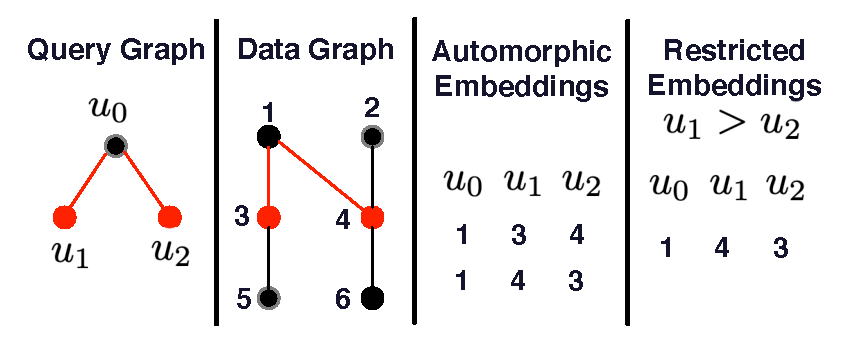
\includegraphics[width=\columnwidth]{./figure/automorphism.eps}
\caption{Examples of automorphic and non-automorphic embeddings.}	
\label{fig:automo}
\end{figure}

If a query graph is symmetric, multiple embeddings can be isomorphic to the same subgraph of the data graph. As shown in Figure
\ref{fig:automo}, the query graph has two symmetric vertices, $u_1$ and $u_2$ and two isomorphic embeddings. We can see in Figure
\ref{fig:automo} that the two embeddings are the same subgraph of the data graph. To eliminate redundant embeddings, GraphPi
\cite{shi2020graphpi} and GraphZero \cite{mawhirter2019graphzero} generate restrictions on query vertices and the corresponding data
vertices in each embedding. Figure \ref{fig:automo} shows that with the restriction $u_1 > u_2$, we can eliminate the redundant embedding.
We use the same method as GraphPi and GraphZero to break the symmetry of a query graph.

\subsection{GPU Architecture}
GPUs are general-purpose massively parallel computing devices. They are widely used to accelerate graph processing tasks, including
subgraph matching \FIXME{\cite{}}. GPU processing units can be abstracted into a two-level hierarchy, the Streaming Multiprocessors (SMs)
and computing cores inside the SM. An SM is further divided into processing blocks. Each processing block contains a fixed number of
threads, called a warp that is the basic scheduling unit.

Modern GPUs also organize their memory into a hierarchical system, containing the global memory, a configurable shared memory, registers,
and potentially an L2 cache between the global memory and the shared memory. The thread-local registers are the fastest memory component,
having the lowest access latency (1-2 cycles). The SM local L1 caches and shared memory provide a larger storage capacity over the
thread-local registers but have modestly higher accessing latency of around 30 cycles. Like the RAM in a CPU system, the GPU’s off-chip
global memory provides the largest memory storage capacity on the GPU but has the most expensive accessing latency of around 500 cycles.

The NVIDIA CUDA programming model provides atomic functions to perform a read-modify-write atomic operation on one 32-bit or 64-bit word
residing in global or shared memory. In this work, we use the CUDA $atomicAdd$ function. This function reads a variable in global memory
before adding a number to it and then writes the result back to the same address.



%GPU has been used in many areas to accelerate applications. The popularity of GPU is primarily attributed to its massive parallelism. To support such large-scale parallelism, GPU employs a complex execution pipeline and memory hierarchy. Modern GPUs usually consist of multiple Streaming Multiprocessors (SMs), and each SM contains multiple Single-Instruction-Multiple-Thread (SIMT) units. Threads in the same SIMT unit are called a warp, the smallest scheduling unit in GPU. The thread-local registers are the fastest memory component, having the lowest access latency (1-2 cycles). The SM local L1 caches and shared memory provide a larger storage capacity over the thread- local registers but have modestly higher accessing latency of around 30 cycles. The off-chip global memory, similar to the RAM in a CPU system, provides the largest memory storage capacity on the GPU but has the longest accessing latency of around 500 cycles.
%
%CUDA provides atomic functions to perform a read-modify-write atomic operation on one 32-bit or 64-bit word residing in global or shared memory. In this work, we use $atomicAdd$ function to read a variable in global memory and add a number to it, and write the result back to the same address.
